% !TeX root = ../index.tex
\chapter{Testing}
\graphicspath{{4-testing/images/}}

I have tested the apps' functionality on a physical device running 6.0 Lollipop (SDK 23) and on two emulated devices:

\begin{itemize}
  \item A Nexus 4 running 4.2 Jelly Bean (SDK 17) as per the minimum requirements, which has a much smaller screen size than the physical device I tested with during the implementation stage.
  \item A Pixel 2 XL running 9.0 Android P developer preview (SDK 28).
\end{itemize}

All three of the devices I tested handled as expected with no compatibility issues found. The styling was also consistent with all three android versions, except a single instance where the tap background animation of icons in the toolbar are square on Jelly Bean instead of circular. The app works in landscape and portrait orientation.

\begin{figure}[H]
  \begin{subfigure}{.5\textwidth}
    \caption{Initial App Installation}
    \centering
    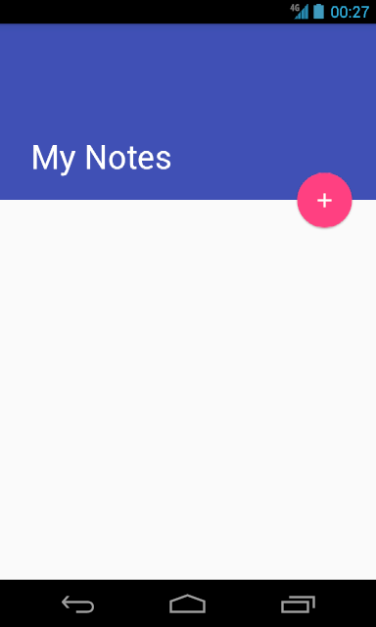
\includegraphics[width=\textwidth]{17-1-initial}
  \end{subfigure}
  \begin{subfigure}{.5\textwidth}
    \caption{Adding a new note with no title}
    \centering
    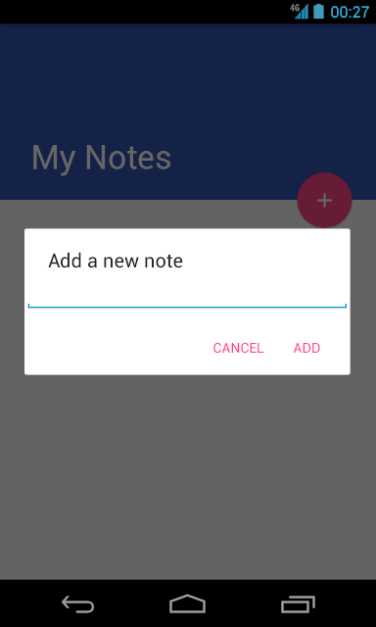
\includegraphics[width=\textwidth]{17-2-newnote}
  \end{subfigure}
\end{figure}

\begin{figure}[H]
  \begin{subfigure}{.5\textwidth}
    \caption{New note created}
    \centering
    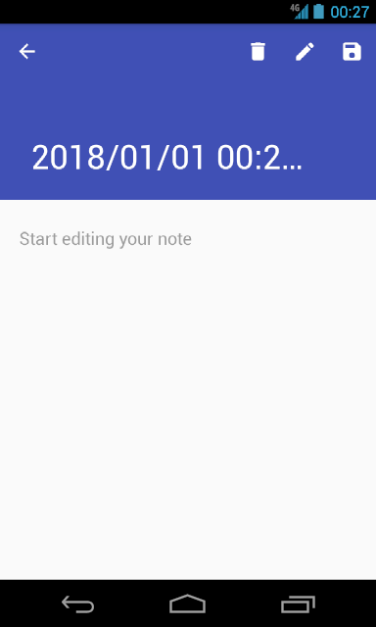
\includegraphics[width=\textwidth]{17-3-newnoteopen}
  \end{subfigure}
  \begin{subfigure}{.5\textwidth}
    \caption{Writing in the note}
    \centering
    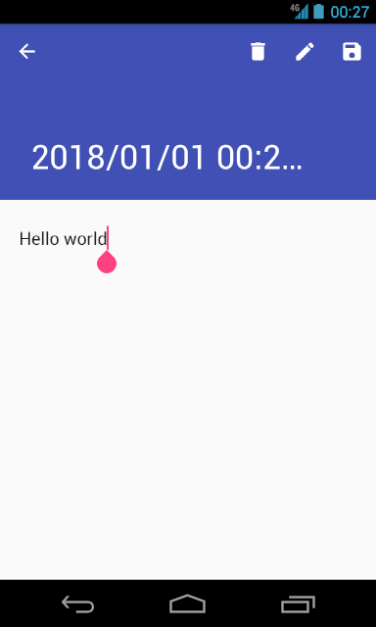
\includegraphics[width=\textwidth]{17-4-editnote}
  \end{subfigure}
\end{figure}

\begin{figure}[H]
  \begin{subfigure}{.5\textwidth}
    \caption{Saving a note}
    \centering
    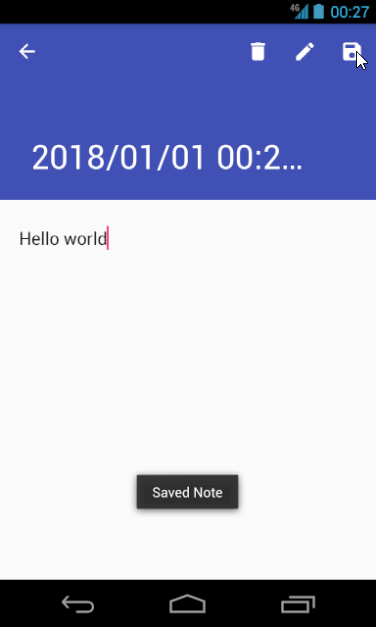
\includegraphics[width=\textwidth]{17-5-savenote}
  \end{subfigure}
  \begin{subfigure}{.5\textwidth}
    \caption{Note list populated with newly created note}
    \centering
    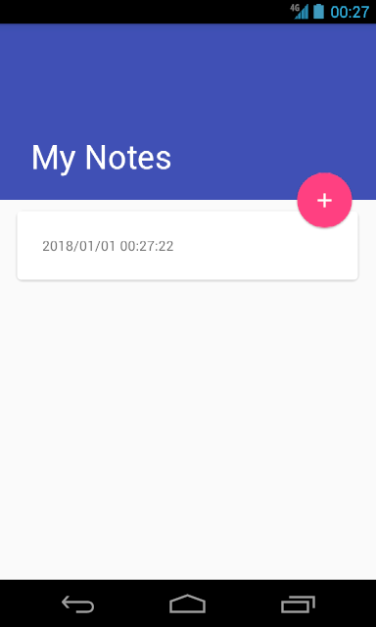
\includegraphics[width=\textwidth]{17-6-notelist}
  \end{subfigure}
\end{figure}

\begin{figure}[H]
  \begin{subfigure}{.5\textwidth}
    \caption{Adding a new note with a title set}
    \centering
    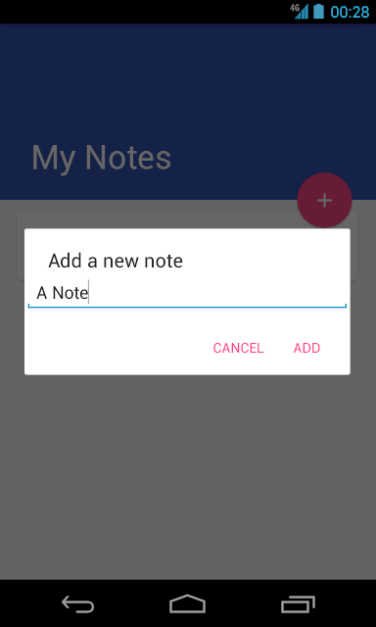
\includegraphics[width=\textwidth]{17-7-notetitle}
  \end{subfigure}
  \begin{subfigure}{.5\textwidth}
    \caption{Editing the note title (middle icon)}
    \centering
    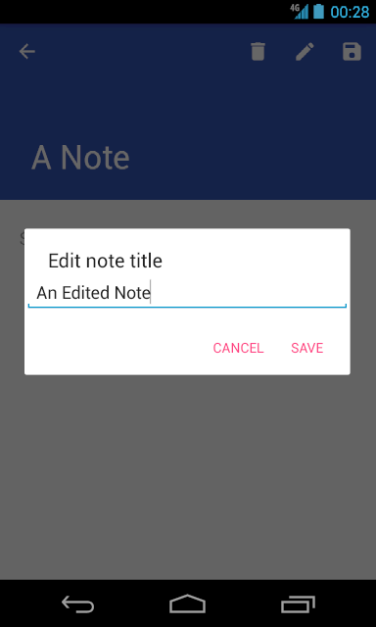
\includegraphics[width=\textwidth]{17-8-editnotetitle}
  \end{subfigure}
\end{figure}

\begin{figure}[H]
  \begin{subfigure}{.5\textwidth}
    \caption{Edited title displayed in note list}
    \centering
    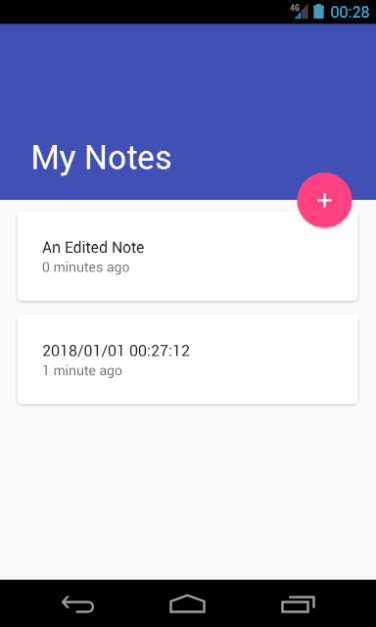
\includegraphics[width=\textwidth]{17-9-updatedlist}
  \end{subfigure}
  \begin{subfigure}{.5\textwidth}
    \caption{Deleting a note}
    \centering
    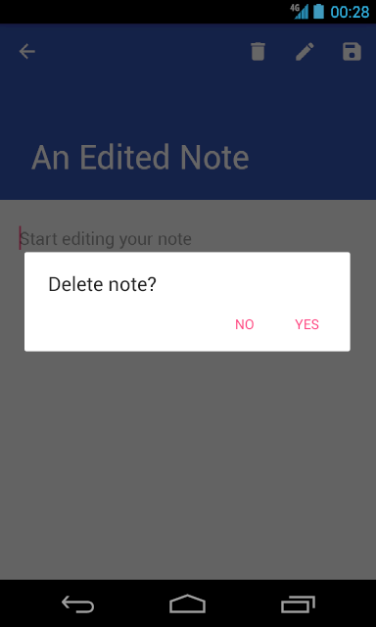
\includegraphics[width=\textwidth]{17-10-deletenote}
  \end{subfigure}
\end{figure}

\begin{figure}[H]
  \caption{Successful deletion of a note}
  \centering
  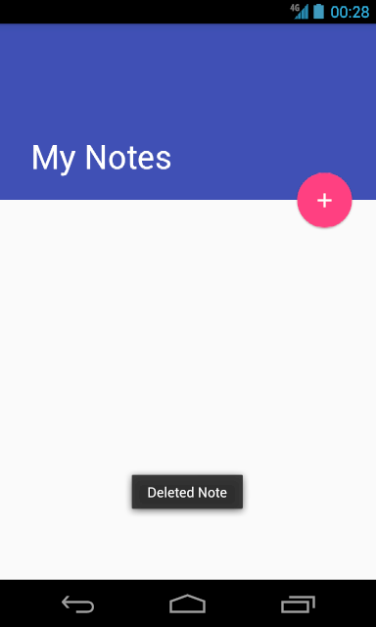
\includegraphics[width=.5\textwidth]{17-11-deletesuccess}
\end{figure}

\begin{figure}[H]
  \caption{Landscape note list}
  \centering
  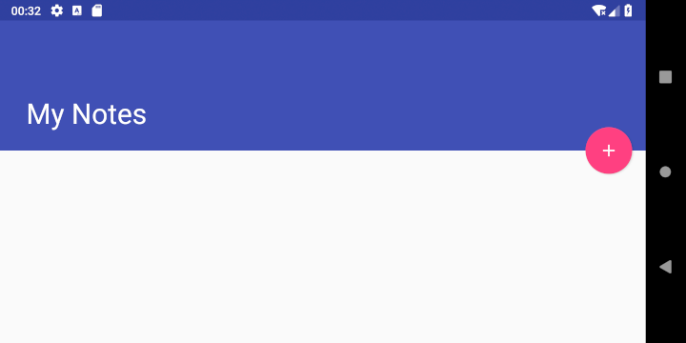
\includegraphics[width=\textwidth]{27-landscape}
\end{figure}

\begin{figure}[H]
  \caption{Landscape note editor with keyboard active}
  \centering
  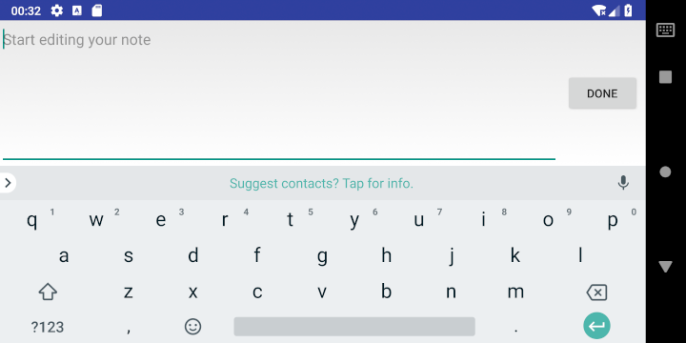
\includegraphics[width=\textwidth]{27-edit}
\end{figure}

\begin{figure}[H]
  \caption{Landscape note activity}
  \centering
  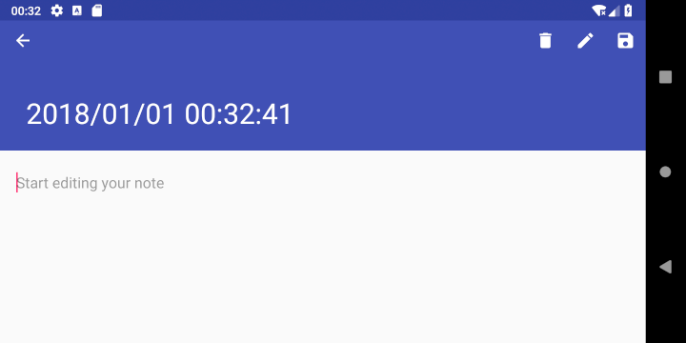
\includegraphics[width=\textwidth]{27-preview}
\end{figure}
